%%%%%%%%%%%%%%%%%%%%%%%%%%%%%%%%%%%%%%%%%%%%
% Introduction
%%%%%%%%%%%%%%%%%%%%%%%%%%%%%%%%%%%%%%%%%%%%




\section*{Foreword}
\addcontentsline{toc}{section}{Foreword}

Looking at the four fundamental forces, gravity is probably the one that we, as a species, take the most for granted. Of course, few of us stop and meditate on the strong and nuclear forces on a daily basis, but we never experience their direct effect. We do not feel the strong nuclear force tying together the protons inside our bodies,  neither do we feel the weak nuclear interaction inducing our potassium atoms to decay into calcium. The electromagnetic force is more present in our mind on a daily basis. Even more so since the arrival of the \textit{f\'ee \'electricit\'e} in our lives and the advent of her child, the electronic age. Even though some manifestations of the electromagnetic force, such as sunlight, are taken for granted, humans keep a sense of wonder about electromagnetism. Magnets, lightning, electromagnetism \textit{feels} magical, as humans have only understood it for a few generations.

What about gravity ? Gravity is part of our mental landscape, we experience its direct effects all the time. If we drop something, it falls, if we throw something, it curves back to the ground, we know this, instinctively. The absence of gravity feels much stranger as our brains evolved under the influence of this fundamental force. Thus we rarely reflect on it. 

However, it is by no means the least interesting of forces.
 
Gravity is the Great Herder, the maker of galaxies, the creator of stars and author of planets. It brings matter together.  

\newpage


\section{From Aristotle to GPU computing : an history of physics and gravity}

\subsection*{Motion}
For two thousand years, Aristote physics dominated european philosophy. Rocks fell to the ground because they wanted to join their element, objects in the sky were attached to eternal rotating crystal spheres, and motion was either natural or violent, the latter needing a continuous force to exist. As the importance of projectiles grew in middle-age warfare, some improvement were made to explain trajectories, such as the impetus, a "contained source of motion" imprinted to a projectile by the thrower. Introduced by Philopon in the 6th century and relayed by Avicenne in the 11th century, it was properly formalized by Jean Buridan in the 14th century in his "Questions on Aristotle's Metaphysics". Buridan's impetus had a lot in common with momentum, in that it was proportionnal to mass and velocity, but could be circular, as shown by this description of celestial motion from Buridan \citep{Clagett1959}:

\begin{quote}
God, when He created the world, moved each of the celestial orbs as He pleased, and in moving them he impressed in them impetuses which moved them without his having to move them any more...And those impetuses which he impressed in the celestial bodies were not decreased or corrupted afterwards, because there was no inclination of the celestial bodies for other movements. Nor was there resistance which would be corruptive or repressive of that impetus.
\end{quote} 


Despite the conceptual mistake of a circular momentum, Buridan, with this text, is the first to include the motion of celestial bodies in the same framework used for everyday, terrestrial motion. The impetus is not a good model, but it is a model for everything in the universe. No more eternal crystal spheres, everything in the universe must obey the same laws. Scientific revolutions do not happen in a vacuum: Buridan and others paved the way for the intellectual landslide of the 16th and 17th century.

\subsection*{Geocentrism and heliocentrism}

While the concept of motion was slowly being refined, our vision of the universe was undergoing some faster changes. The dominant system in Europe since 150AD was the Ptolemaic geocentric model: the Sun and planets went around the Earth, following convoluted trajectories made of circles within circles called epicycles. Though complex, this system was consistent with Aristotle principles of celestial spheres and was accurate to a reasonable extent. Some alternate geocentric models were proposed by arab astronomers, such as Nasir ad-Din at-Tusi and Ibn al-Shatir, as well as rejected attempts to heliocentric models.

Nicolaus Copernicus studied astronomy in Cracow and Bologna, under the influence of hard critics of the ptolemaic system. Strangely, this criticism was not fueled by observations, but by astrology. Astronomy and astrology were closely intertwined, and the chaotic structure of the ptolemaic system made astrological considerations complicated \citep{Barker2014}. In a quest for consistency and simplicity, Copernicus proposed his heliocentric system, published in \textit{De revolutionibus orbium coelestium} in 1543, the year of his death, in which all planets went around the sun, in the correct order. However, clinging to circular orbits, Copernicus had to preserve ptolemaic workarounds such as epicycles. 


\begin{figure}
\center
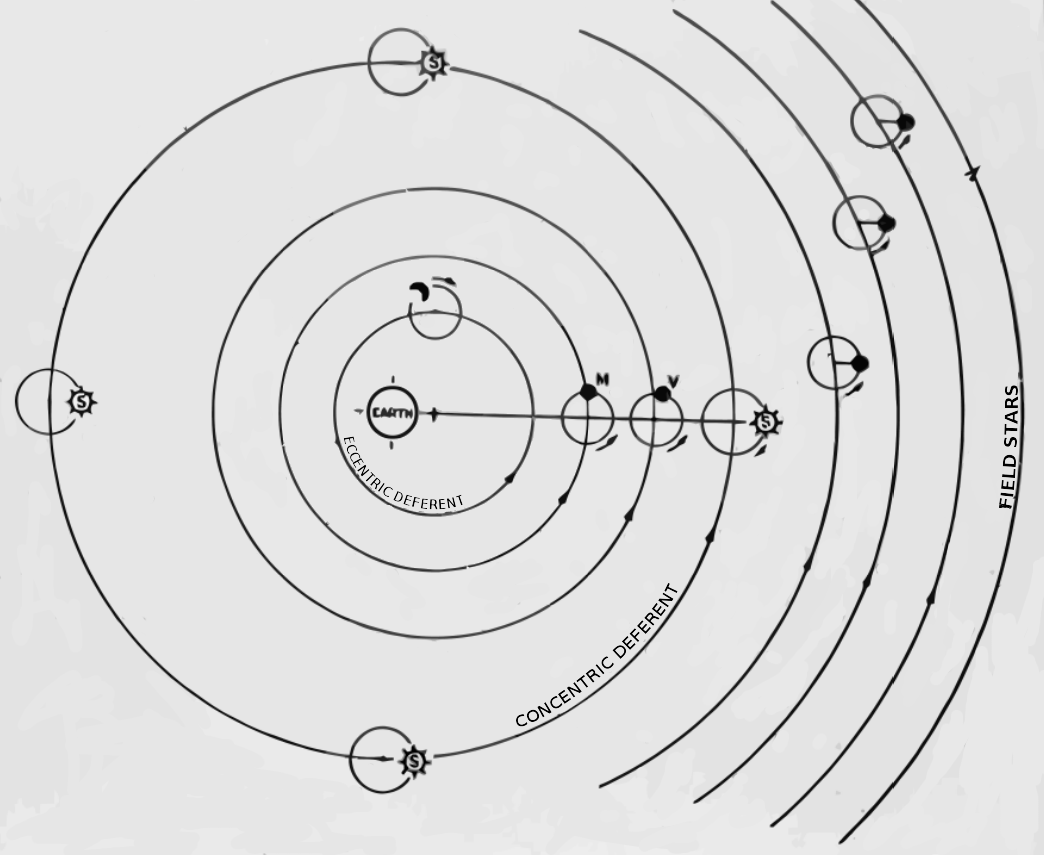
\includegraphics[width=0.45\linewidth]{Figures/0_PtolemaicModel.png}
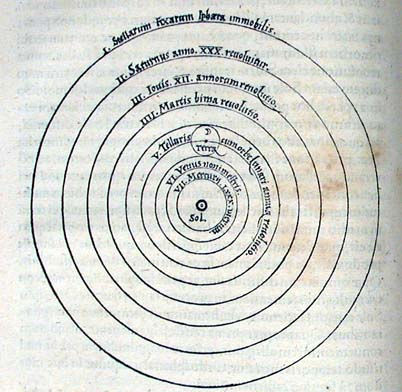
\includegraphics[width=0.38\linewidth]{Figures/0_CopernicusModel.jpg}
\caption{ Left: Depiction of the Ptolemaic geocentric system, the equant is not shown . Right: Copernicus illustration of his own heliocentric system, from \textit{De revolutionibus}. }
\label{Fig:0_PtolemyCopernicus}
\end{figure}



The astronomical evidence was, at the time, paradoxically against him. The apparent size changes of planets could not be measured yet, as well as stars parallaxes, contradicting heliocentrism. The idea of a moving Earth implied some effect on falling bodies (known today as coriolis effect) which were also not measurable at the time. Building on this apparent counter-evidence and on the work of indian astronomer Nilakantha Somayaji, Tycho Brahe, the most renowned astronomer of his time, proposed an alternative model known as the Tychonic system in the late 16th century \citep{ramasubramanian1998}. Brahe maintained the Earth as the center of the universe, circled by the sun, itself orbited by all other planets. The system was very efficient and was quickly adopted by the Church and considered in compliance with the Holy Scriptures.

However, the seed of heliocentrism was planted in european scientific minds. The idea exalted the impetuous and visionnary Giordano Bruno, who pushed the decentralization of Earth to the extreme, claiming stars were other suns, harboring other planets, which themselves could sustain intelligent life. For this, his rejection of catholic dogma and his vehement refusal of retractation, Bruno was burned at the stake on the Campo de Fiori in 1600. Bruno, the fiery dialectist, despised geometry and believed the mind alone could unravel any mystery. 

Johanes Kepler believed in geometry, in consistency and in observations. Ardent supporter of copernicism, he convinced Tycho Brahe to grant him access to his astronomical data, unsurpassed at the time. Focusing on the motion of Mars, Kepler, through trial and error, found out the planet was moving around the Sun following an ellipse. He formulated his first two laws of planetary motions. Further exploration led him to the third law. The three laws of Kepler were formulated, initiating the mathematisation of astronomy, and with it of all physics.

\subsection*{The Starry Messenger}


The father of modern astronomy, and precursor of modern science, Galileo Galilei was born in Pisa in 1564. For the first part of his scientific career, Galileo got famous for his lectures on mechanics and motion. Building on Buridan and Oresme's ideas, he expressed the mathematical form of free fall motion $ d = \frac{gt^2}{2}$. Galileo also formulated what was essentially the future first law of motion from Newton.

In 1609, his passion for scientific instruments led Galileo to build his own "dutch perspective glass", or telescope, a pioneering optical device from the netherlands. Once pointed at the sky, the device triggered an avalanche of observations who would forever bury the aristotelitian view of perfect and unchanged heavens. Moving Jupiter satellites, Moon craters and mountains, millions of stars in the Milky Way, these were consigned into \textit{Sidereus Nuncius} (Starry messenger), the first scientific publication of astronomical observations \citep{galileo1610}.

Strong advocate of copernicism, but lacking proper evidence, Galileo caused a large controversy with his 
\textit{Dialogue Concerning the Two Chief World Systems} published in 1632, a pamphlet against the ptolemaic system, presenting (arguably unintentionnaly) one of its advocates as a simpleton. Despite his friendship with the pope, he had to retract his work and reject copernicism. Galileo spent the rest of his life on house arrest. Observationnal evidence at the time was still on the side of geocentrism, but the extent of the backslash against Galileo showed the febrility of a Church having absorbed Ptolemy and Aristotle principle into its doctrine, in a time where the debate was shifting from theology to physics and observations.

The relativity of motion is often attributed to Galileo, as he includes it in its controversial pamphlet, stating that a traveller inside a ship sailing smoothly would not be able to tell he's moving. Thus, people could be standing on a moving Earth without feeling it. However, this thought experiment was nothing new at the time and had been a recurring theme of mechanical philosophy since Buridan. Oresme, Copernicus and Bruno had been building on the idea, expanding and improving it, developing over the centuries an implicit understanding of inertia, until Bruno actually gives it a name: \textit{virt\`u}. Galileo may have met Bruno himself, and had surely been influenced by his writings \citep{DeAngelis2015}. Galileo's formulation was clearer, and part of a larger understanding of motion, introducing the concept of reference frame. After Copernicus decentralized the Earth, Galileo decentralized human subjectivity itself, setting the scene for the revolution to come. 

\subsection*{On the shoulders of giants}

Isaac Newton is without a doubt the father of modern mathematical science. Admitted in Cambridge in 1661, Newton supplemented the -still- official aristotelitian teaching with more modern authors: Copernicus, Galileo, Kepler, and most of all, Descartes. The french philospher had a profound impact on the young student, rooting his love for mathematics and deductive reasoning. However, while Descartes showed disdain for experimentation, Newton was an acute observer of the natural world. 

In 1666, while in is mother's farm, having been forced out of Cambridge by the Plague, Newton began his reflexion on the motion of celestial bodies. He derived from Kepler's law that the Sun had to exert an inverse squared distance attraction on the planets. Extending the concept to the Earth, moon, and a famous apple, Newton found a way to verify his hypothesis, using data from Galileo mechanical studies on the strength of Earth attraction. The wrong estimate of Earth radius he used at the time introduced a discrepancy which put the young man off his \textit{gravitas} studies for 18 years.

Edmond Halley, astronomer and friend of Newton, having heard of Newton inverse squared law, urged him in 1684 to communicate his work the Royal Society. With a new accurate measure of Earth radius and confronted to a concurrent claim to his law from Robert Hooke \citep{Kramer1982}, Newton capitulated to Halley's eager enthousiasm and communicated his work in the famous \textit{Philosophiæ Naturalis Principia Mathematica} \citep{Newton1687}. Published at Halley's own expense, the Principia shook all of Europe. Newton had invented Calculus (in parallel of Leibniz) and applied it to derive the universal law of Gravitation.

\begin{equation}
F = G \frac{m_1.m_2}{r^2}
\end{equation}


Where:
\begin{itemize}
 \setlength\itemsep{-0.5em}
  \item[$F$] Gravitational attraction between object 1 and object 2
\item[$G$] Gravitational constant, $6.67408.10^{-11} m^3 kg^{-1} s^{-2}$ \citep{Pavese2015}
\item[$m_i$] Masses of object 1 and 2
\item[$r$] Distance between object 1 and 2
\end{itemize}

Though Newton was part of continuous line of geniuses and innovative minds building from each others, as he puts it "If I have seen further it is by standing on the shoulders of giants" \citep{Maury1992}, his input was truly revolutionnary. He made large advances in optics and mathematics, and created a consistent mathematical framework to compute motions, essentially founding modern science and sowing the seeds of the industrial revolution. This framework is summed up by Newton's three laws of motion (from recent translation \citealt{Cohen1999}):

\begin{quote}
Law I : Every body persists in its state of being at rest or of moving uniformly straight forward, except insofar as it is compelled to change its state by force impressed.
\end{quote}

\begin{quote}
Law II: The alteration of motion is ever proportional to the motive force impress'd; and is made in the direction of the right line in which that force is impress'd.
\end{quote}
 
 \begin{quote}
 Law III: To every action there is always opposed an equal reaction: or the mutual actions of two bodies upon each other are always equal, and directed to contrary parts.
 \end{quote}

The second law can be mathematically formulated in more modern terms:

\begin{equation}
\sum \bold{F} = \frac{d \bold{p}}{dt}
\end{equation}

Meaning the sum of all forces $\bold{F}$ applied to an object is equal to the time derivative of its momentum $\bold{p} = m.\bold{v}$.



\subsection*{The n=3 body problem}

As the Enlightenment brought a scientific revolution in many fields, I will now limit the discussion to the development of celestial mechanics, while acknowledging input from other fields.

While the two-body problem had been solved by Newton and expanded by Bernoulli in 1710 \citep{Barrow1997}, in the 18th century the three-body problem remained the object of much investigation and development. A general solution for the Earth-Moon-Sun system would have had applications on nautical astronomy and trans-continental navigation. Extended analytical work by d'Alembert, Clairaut, Euler and Lagrange led to the development of early families of approximate solutions or exact solutions to special cases.

From 1773 to 1793, Joseph-Louis Lagrange, helped by his invention of Lagrangian mechanics, would make a lot of advances on the three-body problem. He introduced the concept of potential and discovered libration points (later known as Lagrange points). In the same time, Pierre-Simon de Laplace proved the stability of the solar system using a newly developped perturbation theory. The solar system dynamics were being unraveled, with finely tuned perturbation computation, but the general three-body problem remained unsolved.

In 1888, Henri Poincaré, greatest mathematician of his time, submitted an entry to a contest organized by the King of Sweden Oskar II. The goal was to determine a usable solution to the n-body problem, for any given n. While Poincaré does not submit a complete solution, he wins the contest by presenting an in-depth exploration of the phase-space of the restricted three-body problem, which would later give rise to the Chaos theory ,see \cite{Yoccoz2010}. Poincaré managed to prove that the three-body problem had no  solution involving simple functions.

Contrary to popular belief, the three-body problem \textit{has} a solution, it was derived by Karl F. Sundman in 1912 \citep{Sundman1912}. However, any attempt to obtain accurate trajectory predictions would face tremendous convergence time and is in practice unusable \citep{Beloriszky1930}.

It is interesting to note that Elis Str\"omgren performed by-hand calculation of a three-body system, see \cite{Aarseth2003,Stromgren1909}, prefiguring the advent of numerical orbit computation.

\subsection*{The n$>$3 body problem}

\begin{quote}
"The Sun attracts Jupiter and the other planets, Jupiter attracts its satellites and similarly the satellites act on one another."
\end{quote}

By this sentence from the \textit{Principia}, Newton formulates the n-body gravitational problem, an arbitrary number of massive bodies all interacting gravitationally, for the solar system. The "n$>$3-body" problem didn't receive a lot of attention at first, as the unruly three-body problem was on everyone's mind, and a n$>$3-body problem seemed abstract, the solar system example being appropriatly dealt in approximations.

In 1764, Charles Messier resolved individual stars in Messier 4, a globular cluster, hundreds of thousands of stars grouped together. Many new clusters were to be found afterwards, extending the catalog of real-life n-body systems. However, nothing was known of their kinematics, the stars were somehow suspended motionless in the sky. This was the case until the advent of Doppler spectroscopy, which allowed astronomer to measure stars velocities \citep{Doppler1842}. Stellar dynamics had begun.

The n$>$3-body problem was still inaccessible, so scientists like James Jeans and Arthur Eddington decided to take the problem from the other hand, and took advantage of the large number of stars. Inspired by \cite{Poincare1906}, both astronomers applied the statistical theory of gas to stellar systems, founding the field of stellar dynamics \citep{Jeans1916,Eddington1916}.

An interesting experiment was conducted by \cite{Holmberg1941} to understand the collision of two stellar systems (galaxies). With too few points to warrant a statistical approach, and before the rise of numerical integration, Holmberg modelled two galaxies with dozens of lightbulbs and photocells, measuring the attractive force with the amount of light received in each direction, taking advantage of the inverse squared fall of luminosity with distance, akin to gravity.

\subsection*{The numerical age}

The first numerical N-body computations were performed by Sebastian Von Hoerner in 1959 when visiting the University of T\"ubingen, on a Siemens 2002, a cutting edge calculator at the time. The very first had N=4. Then, Von Hoerner, back in Heidelberg, worked his way up to 16 stars, then 25, programming and debugging on punch cards. This story was told by Von Hoerner himself in \cite{VonHoerner2001}. He very quickly realized the importance of binary stars and their impact on computations. He was also able to confirm some theoretical prediction on cluster dynamics, and found an interesting radial density profile with a center cusp \citep{VonHoerner1960,VonHoerner1963}.

\begin{figure}
\label{Fig:N_increase}
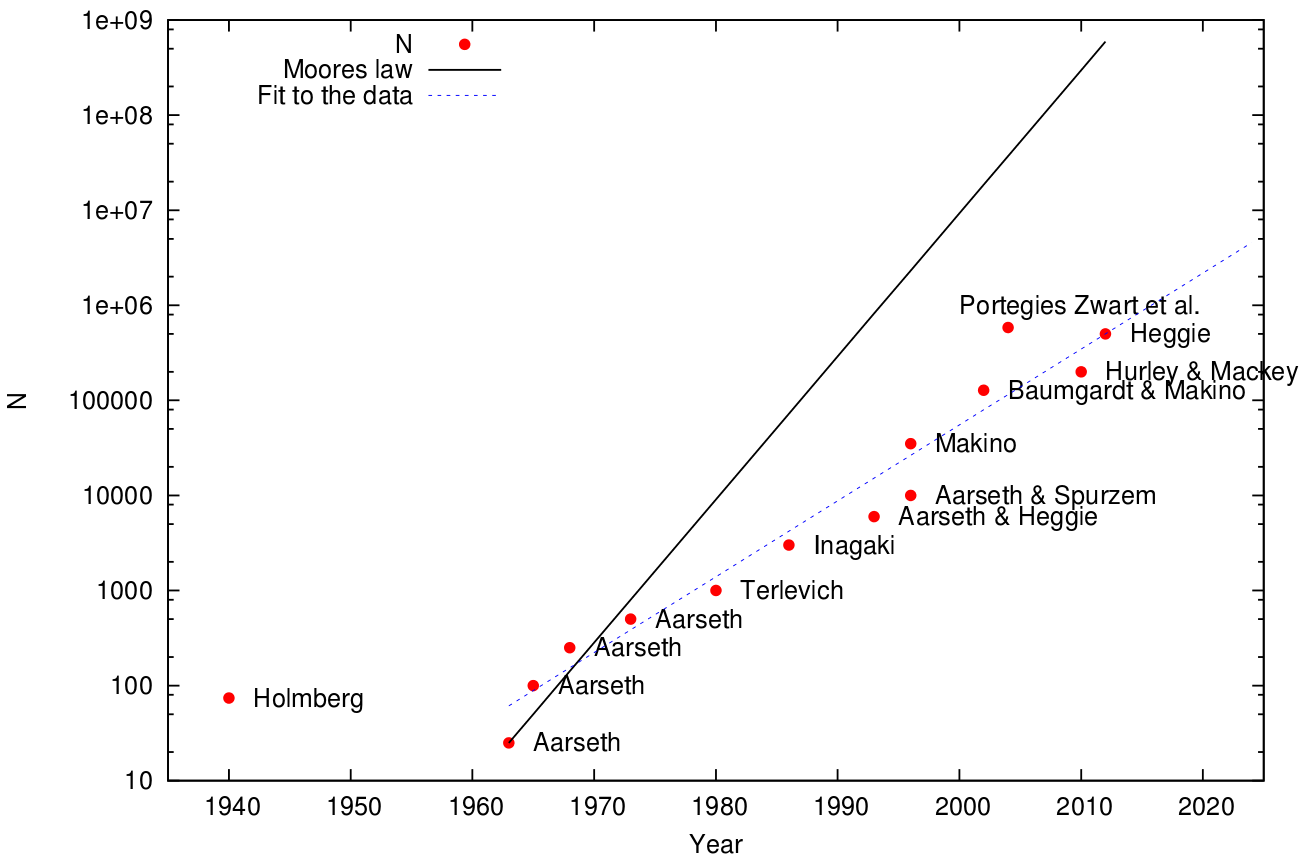
\includegraphics[width=0.9\linewidth]{Figures/0_N_increase.png}
\caption{The evolution of the number of particles in N-body simulations. Solid line shows the Moore law. The figure was taken from \protect\cite{Bedorf2012}. }
\end{figure}


There was two ways to increase the number of stars in simulations: buy a better computer or improve the algorithm. Sverre Aarseth got invested in the second path, which would take over his scientific life. Aarseth pioneered the use of individual time-step, changing the rate at which particles positions are updated, gravitationnal softening, allowing convergence for close approach, and polynomial prediction for force calculations \citep{Aarseth1964}. As power and optimization grew, investigations expanded, such as the interaction star-gas \citep{VanAlbada1968a} and binary formation \citep{VanAlbada1968b}.

The 1970s brought two new important optimisation methods: KS regularization of close pairs \citep{Aarseth1972} and Ahmad-Cohen neighbour scheme \citep{AhmadCohen1973}. The number of stars in simulations kept growing, reaching 1000 with \cite{Terlevich1980} and materializing into the \textit{NBODY5} integrator. At this point various methods departing from a pure collisional calculation began to emerge, such as the simplified distant interaction with the \cite{BarnesHut1986} tree algorithm.

To go beyond the regular improvement of computing power with time, a group of japanese researchers, among whom Junichiro Makino, designed and built special purpose hardware for many-body problems: GRAPE \citep{Ebisuzaki1990,Ito1991}. These cards vastly improved the speed of nbody simulations and were a milestone on the road to the parallelization of computing. With the force calculation directly implemented in the hardware, GRAPE dominated the field for 15 years.

The latest technological leap in Nbody simulations came from graphic cards, see \cite{Bedorf2012} for a more detailed historical perspective. Graphical Processing Units, or GPU, were originally designed for computer games visual rendering, applying the same transformations to a lot of pixels at the same time. These made them very efficient parallel computing machines for physics. Interest in GPU computing started to grew in the 2000s \citep{Nyland2004,Elsen2006,SPZ2007} until the advent of usable GPU programming languages, like CUDA, in the late 2000s. At this point GPU were more efficient than GRAPE hardware for force calculation. Keigo Nitadori and Sverre Aarseth developped a GPU-accelerated version of the latest NBODY code, NBODY6, in 2012 \citep{Nitadori2012}.

Last year, 329 years after the publication of the \textit{Principia}, a collisional nbody simulation of one million stars was performed with a modified version of NBODY6 running on GPU \citep{Wang2015}. Computers have made it possible for humans to study systems of incredible scales in space and time, only using the universal law of gravitation. N-body numerical integrators are the culmination of centuries of scientific development on the motion of massive bodies.



\newpage
\section{Star clusters}

\subsection{What are star clusters ? And why study them ?}

The widest definition possible for a star cluster is "An area of the sky with visibly grouped stars". However, this includes binary stars and galaxies. We are interested in intermediate systems, such as open clusters, globular clusters or associations, in which stars are, if not bound, at least under direct mutual gravitational influence. These objects can either dissolve in less than a million year or remain bound for billions of years.

Clusters are the result of bursts of star formation in Giant Molecular Clouds. All stars within a cluster were born approximately at the same time, which explains the sustained interest of the scientific community for star clusters for more than a century. They are the best laboratories of stellar physics available to us: a large population of stars sharing the same age and distance to Earth. The age of the cluster can be derived from the most massive stars in the population, as stars have lifetimes inversely correlated with their mass. Overall, integrated spectral features from all members of a star cluster can provide a wealth of information.


\begin{figure}
\center
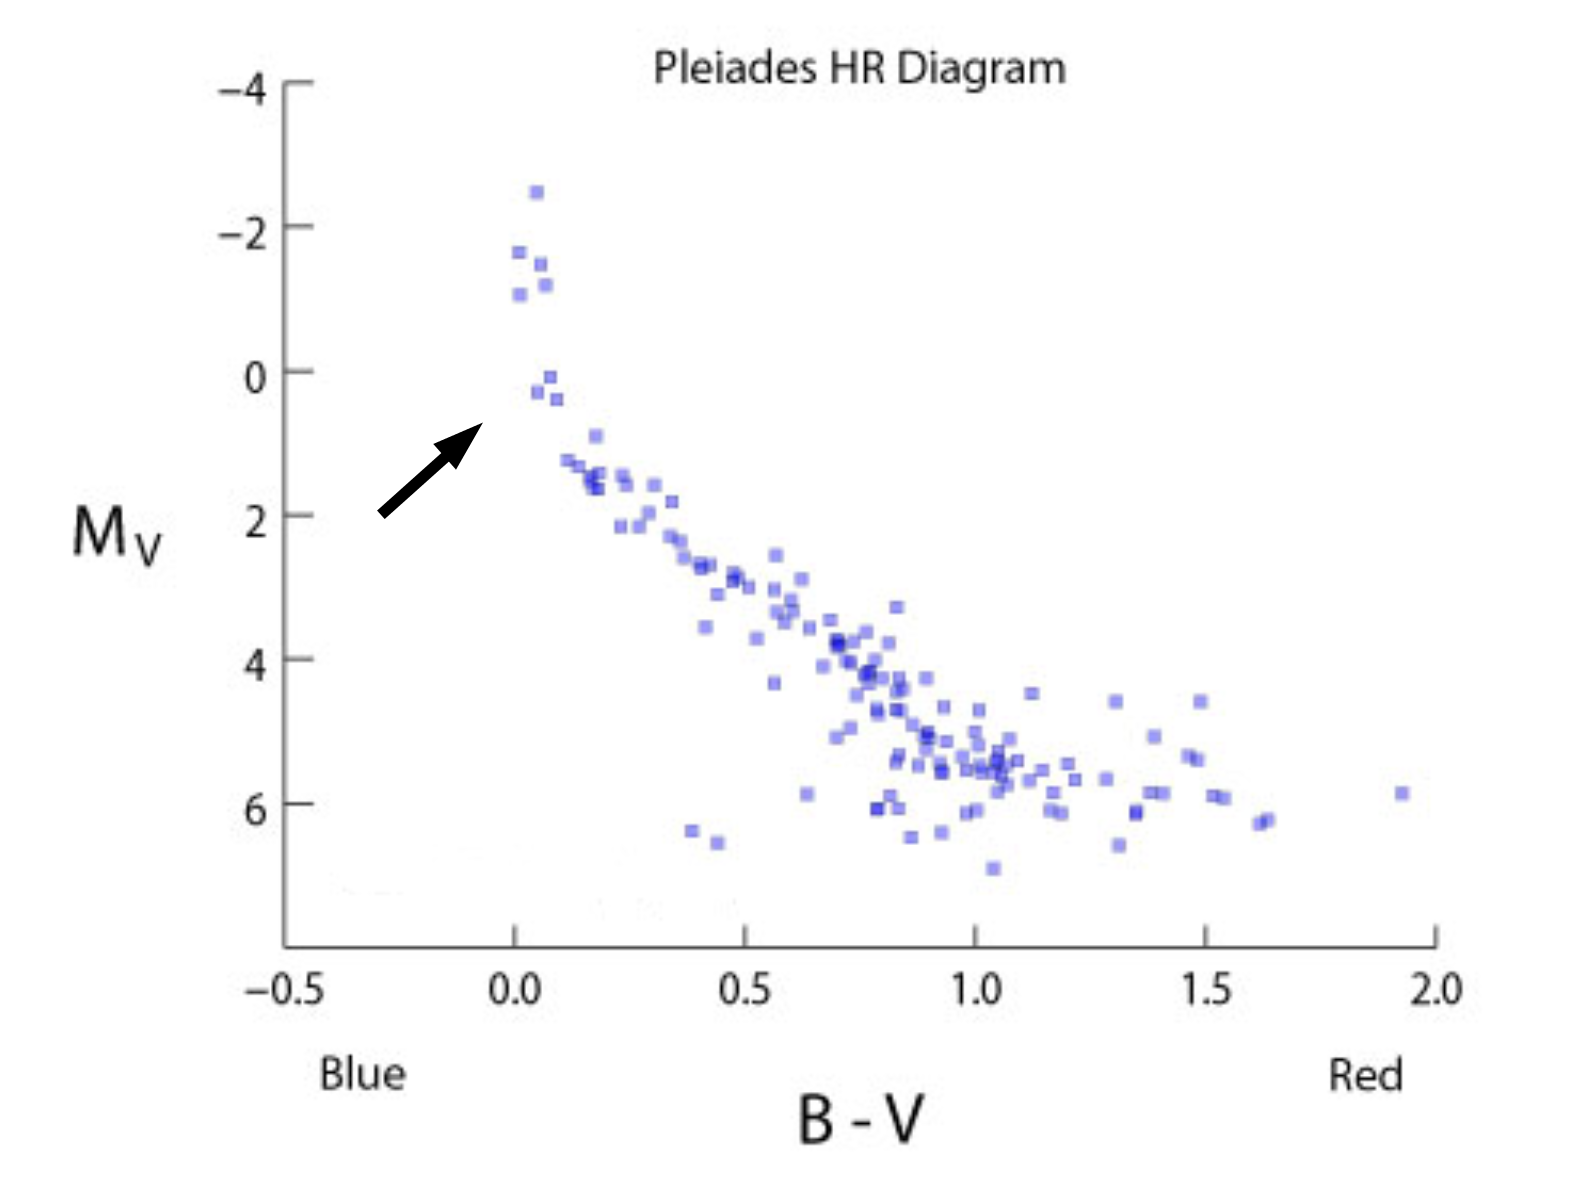
\includegraphics[width=0.45\linewidth]{Figures/0_HRDiagram_Pleiades.png}
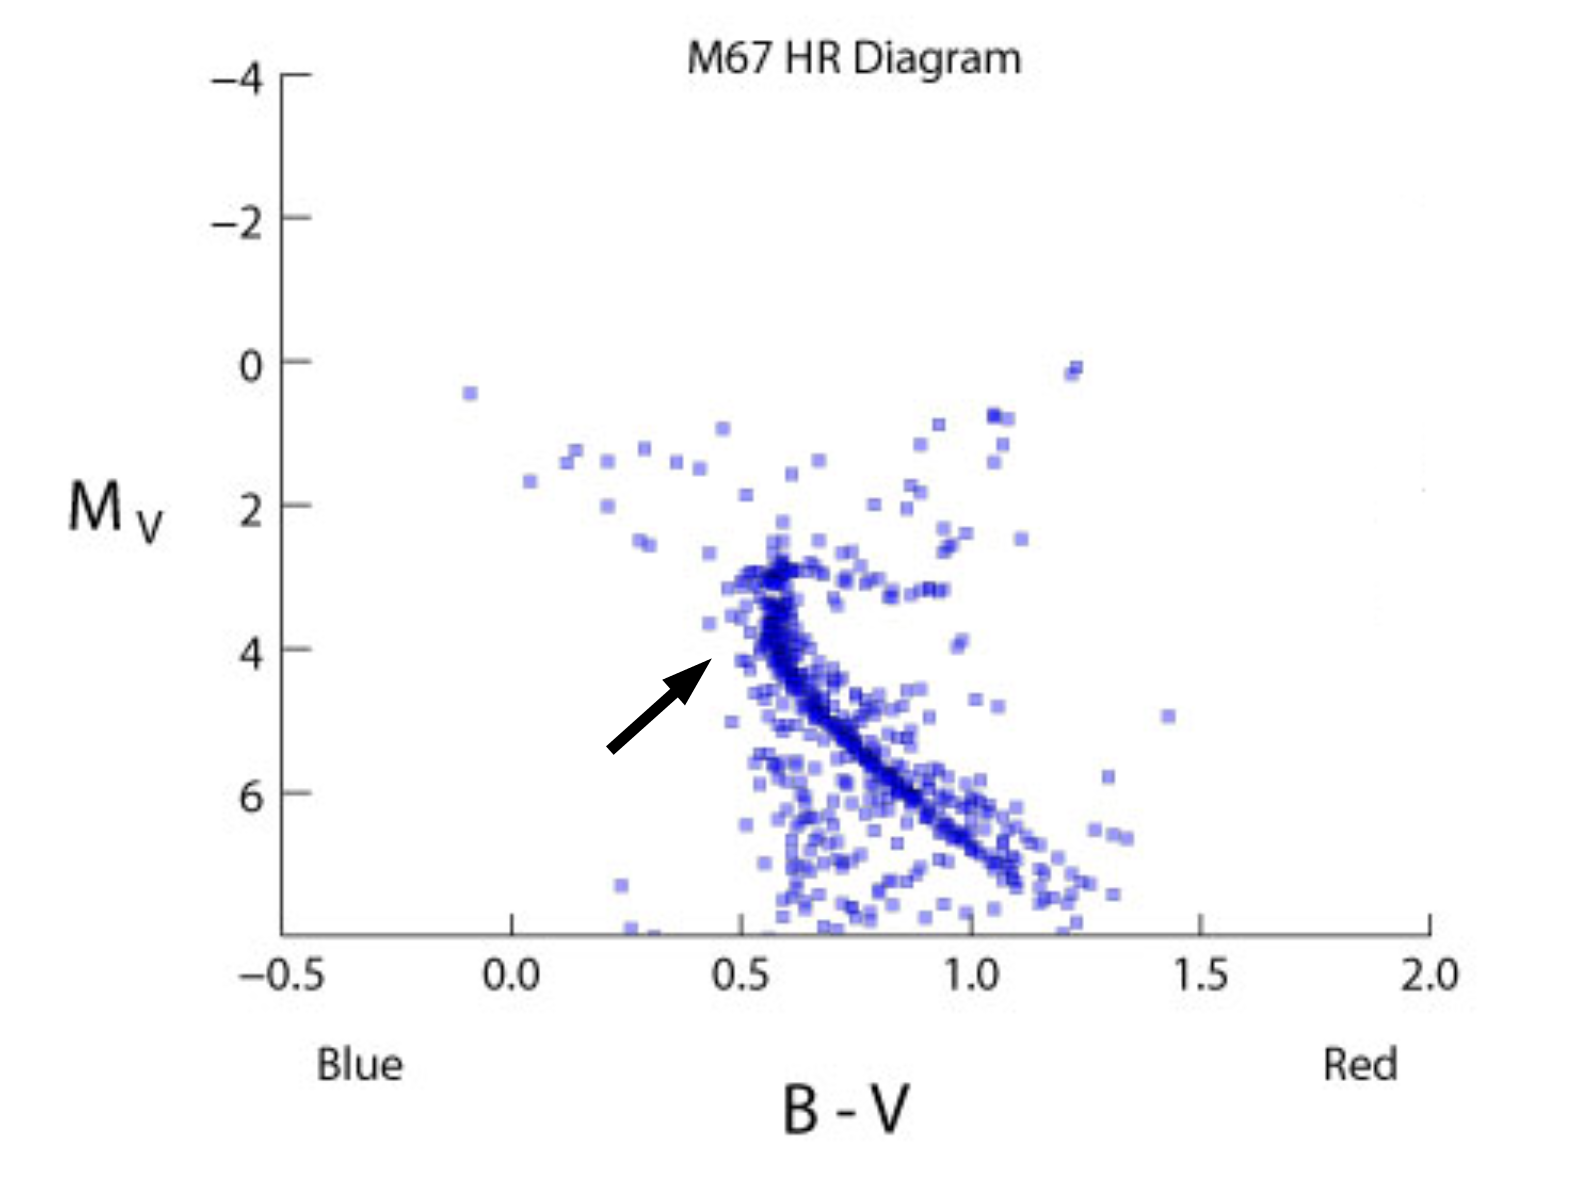
\includegraphics[width=0.45\linewidth]{Figures/0_HRDiagram_M67.png}
\caption{Hertzprung-Russel diagram of the Pleiades and M67. An arrow points at the Main-Sequence turn-off for each cluster. The figures were taken from the \href{http://www.astrophysicsspectator.com/topics/stars/HertzsprungRussellClusters.html}{Astrophysics Spectator} website and data can be found in \protect\cite{Stassun2002,Kharchenko2004}  }
\label{Fig:0_HR}
\end{figure}

One example is the ability to date a cluster, thus its members, through the main-sequence turn off. On figure~\ref{Fig:0_HR} is shown the Hertzprung-Russel diagram for two different clusters: The Pleiades and M67. The HR diagram shows the luminosity of the star versus its color, redder on the right, bluer on the left. Stars spend most of their life on the Main Sequence, with the most massive, luminous blue stars on the left, and red fainter smaller stars on the right. Massive stars have shorter lives and depart from the main sequence before small stars. Looking at the Main Sequence turn-off in the HR diagram of a cluster tells us the mass of the stars currently leaving the MS, which gives its age and that of all other stars. As seen on the figure, the Pleiades are younger (100Myr) than M67 ($\sim$ 4 Gyr) as the stars leaving the MS are more massive.

Star clusters are historically divided into two main categories: globular clusters and open clusters. As observationnal techniques improve, categories tends to blend into a spectrum of size, age, and dynamical state, with Young Massive Clusters, embedded clusters, associations.






\subsubsection*{Globular clusters}

Globular clusters are old and massive stellar systems. Most of them are older than 10 Gyr and more massive than $10^4~M_\odot$. They only contain stars, with no dust or gas. The 150 known globular clusters in the Milky way are scattered in the disk and the halo. Due to their age, GCs are dynamically evolved. Introducing the relaxation time, defined in \cite{BT} by:
\begin{equation}
\label{Eq:0_relaxation}
t_{relax} = 0.1 \frac{N}{logN} t_{cross} = 0.1 \frac{N}{logN} \frac{R_{hm}}{\sigma}
\end{equation}

with $t_{cross}$ the crossing time, defining the time a star takes to cross the system and $\sigma$ the internal velocity dispersion. The relaxation time is the time it takes for a system to erase its initial condition, perturbation per perturbation. GCs have a relaxation time of about a Gyr, they are relaxed systems. Various models have been put forward for the structure of GCs, the King \citep{King1966} and Plummer \citep{Plummer1911} models are the most widely used.




\begin{itemize}

\item 47 Tucanae (NGC 104) is one of the most massive known globular cluster in the Milky Way. It is estimated to contain about 1.5.$10^6~\Mo$ and to be 13 Gyr old\citep{Forbes2010}. Its core is extremely dense, as many GCs, with a central density up to $10^6 \Mo/\textrm{pc}^3$. Such a concentration of stars is a favorable environment for stellar collisions, which create what is called \textit{stellar exoticae}, stellar object not following the standard evolutionnary path, such as blue stragglers. Blue stragglers are stars too luminous and too massive compared to the age of the cluster, likely formed out of colliding stars. 47 Tuc exhibits a population of such objects, as well as others: Cataclysmic variables, X-ray binaries, etc. These are the direct consequence of the very dense environment of globular clusters such as 47 Tuc.

\item Messier 12 (NGC 6218) is on the light end of the mass spectrum with 9.$10^4~\Mo$ \citep{Marks2010}. Such a low mass is however thought to be due to the cluster's dynamical history. Globular clusters have orbits around the galaxy, some more dangerous than others. For example Palomar 5 is currently disappearing after violent encounters with the galactic center. A study by \cite{DeMarchi2006} showed M12's orbit probably also passes close to the galactic center. Subjected to the strong tidal forces of the galactic bulge, M12 would have lost about 4/5 of its original mass. This scenario is backed by the mass function of M12. The mass function is the distribution of stellar masses, and its slope is thought to be more or less universal, though it appears unusually flat in M12. The tidal shock would have preferentially depleted low mass stars, as a process known as mass segregation tends to have massive stars sink at the center and low-mass stars overpopulate the outskirts of the system. 

\item NGC 2808 is reported to contain 1.4 $10^6~\Mo$ \citep{Boyles2011}. NGC 2808, as all others GCs, had long been thought to have an homogeneous stellar population. Yet, a study by \cite{Piotto2007} showed NGC 2808 contained at least three different stellar sequences. As this cannot be explained by the natural age spread arising from a continuous star formation at the birth of the cluster, such observations have far-reaching implication on its formation scenario, and those of many GCs with multiple populations. Several hypothesis are being explored, such as GCs being the outcome of mergers \citep{Pasquato2016} or a sequence of distinct star forming events \citep{Dantona2016}, with no consensus for now.

\end{itemize}


\begin{figure}
\label{Fig:0_GlobularClusters}
\center
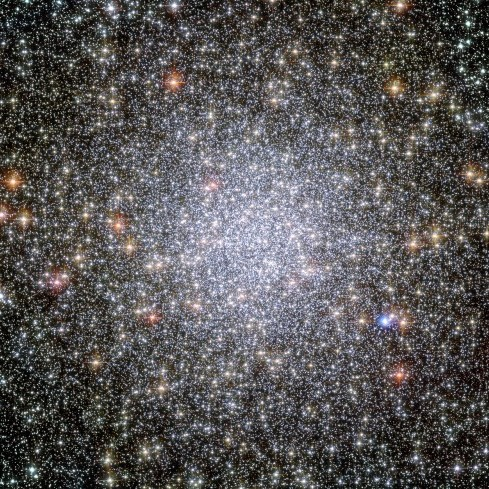
\includegraphics[width=0.3\linewidth]{Figures/0_47Tuc.jpg}
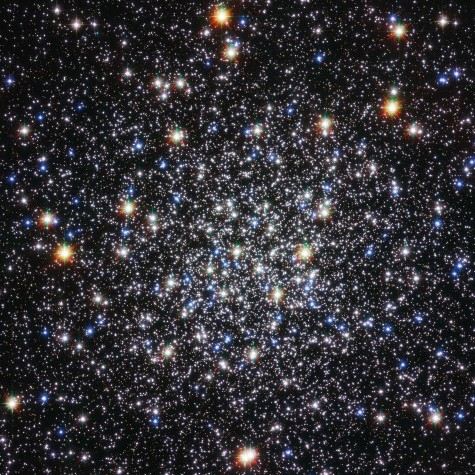
\includegraphics[width=0.3\linewidth]{Figures/0_M12.jpg}
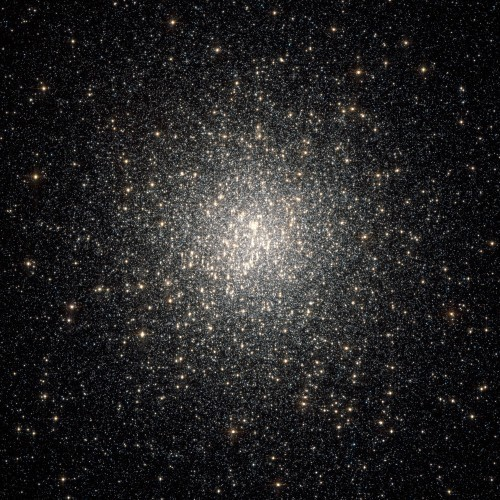
\includegraphics[width=0.3\linewidth]{Figures/0_NGC2808.jpg}
\caption{From left to right: 47 Tucanae, Messier 12 and NGC 2808. Credits: ESA/Hubble. }
\end{figure} 


\subsubsection*{Open clusters}


\begin{figure}
\center
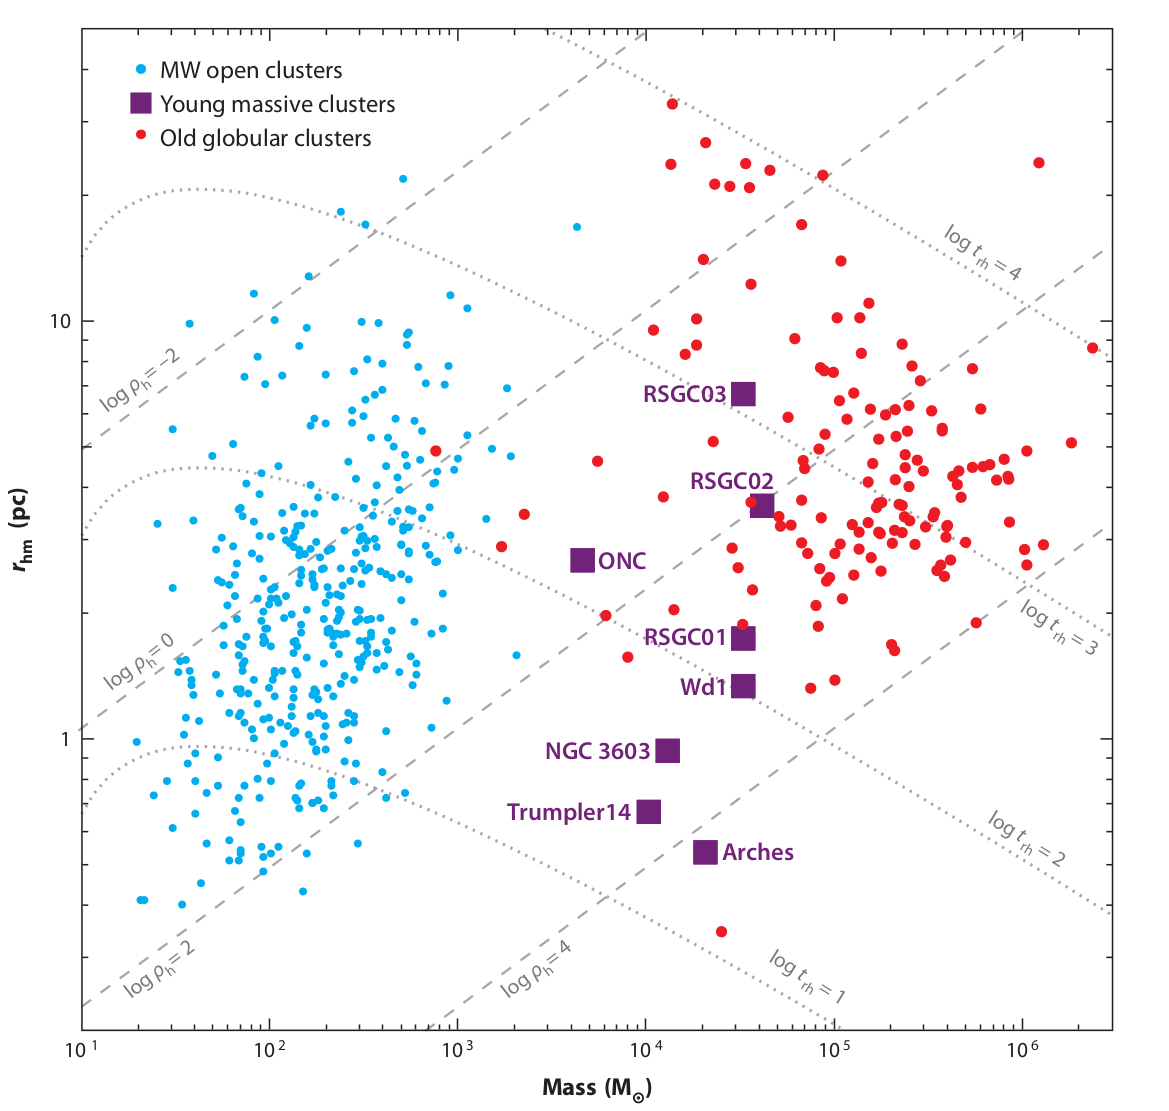
\includegraphics[width=0.65\linewidth]{Figures/0_MassRadiusClusters.png}
\caption{Radius-Mass Diagram for Milky Way clusters. Blue dots are open clusters, red dots Globular clusters and purple squares show Young Massive Clusters. Dashed lines show constant density within half-mass radius $\rho_h = 3M/8\pi r^3_{hm}$ and dotted lines show constant relaxation time. The plot was taken from the review \protect\cite{PortegiesZwart2010}.}
\label{Fig:0_SPZ}
\end{figure}


Open clusters are lighter objects, rarely more massive than $10^3 \Mo$. They are also younger, typically no older than a Gyr. In fact, Open Clusters are thought to be very volatile, with the vast majority not surviving beyond 100Myr. Causes of disruption include internal two-body evolution and tidal shocks from passing massive clouds on nearby orbits.



\subsection{Formation in Giant Molecular Clouds}

\subsection{Early dynamical evolution}

\subsection{Binary stars in clusters}









\newpage
\section{NBODY6}


NBODY6 is the second youngest iteration of the NBODY family, a suite of n-body integrators created by Sverre Aarseth. It can compute the gravitational interaction between up to 128,000 stars in a collisional fashion, meaning there is no softening of the potential, at any scale. This allows for very close binaries to form and remain in the system. To achieve its impressive performances, NBODY6 relies on several optimization technique which have been first developed in the 1960s and 1970s, and improved ever since. Here will be developped four major features of NBODY6, in chronological order of their implementation: block time-step, KS-regularization, Hermite scheme and Ahmad-Cohen neighbour scheme. A full description can be found in Sverre Aarseth's book \citep{Aarseth2003}. Inspiration for this section should be credited to the user manual of NBODY6++, written by Emil Khalisi and Rainer Spurzem.

\subsection{H\'enon units}

NBODY6 uses a set of units specifically invented for the Nbody gravitational problem, the Nbody units, or H\'enon units (as prescribed by Douglas Heggie during the MODEST 2014 meeting). These units are based on three relations:

\begin{align}
G &= 1\\
M_t &= 1\\
E &= -\frac{1}{4}
\end{align}

With $G$ the gravitational constant, $M_t$ the total mass of the system and $E$ total energy of the system. For a virialized system, that is a relaxed system in which the virial ratio 
\begin{equation}
Q = - \frac{E_k}{E_p} = 0.5
\end{equation}
it comes that $E_k=0.25$ and $E_p = -0.5$ and, considering the definition of the virial radius 
\begin{equation}
R_v = - \frac{G M_t^2}{2 E_p} = 1.
\end{equation} 

This unit system was designed for virialized systems, but can be used for out of equilibrium systems, as long as they are bound ($Q <1$), with energy expressions functions of $Q$
\begin{align}
E_p  &= - \frac{1}{4(1-Q)}\\
E_k &= \frac{Q}{4(1-Q)}
\end{align}
which still fulfills the $E = -\frac{1}{4}$ condition. In practice, the H\'enon mass, radius and velocities are obtained through

\begin{align}
m_h &= \frac{m}{M_t}\\
r_h &= 4 (1-Q) |E_p| \cdot r\\
v_h &= \sqrt{ \frac{Q}{4(1-Q) E_k} } \cdot v
\end{align}

which can be used as an input for NBODY6.
\subsection{Block time-step}
 
In the first Nbody simulations, the system was integrated with an universal time-step, determined by the most accelerated star. A star in the outer regions of the cluster with a small velocity did not need to be updated that often. One of the first improvement  was the introduction of individual time-step: each star is attributed its own time-step, depending on the force that is applied to it and its derivative:

\begin{equation}
\label{Eq:0_timestep}
\Delta t_i =  \eta \sqrt{\frac{ |\bold{F_i}||\bold{F^{(2)}_i}| + |\bold{F^{(1)}_i}|^2 }{|\bold{F^{(1)}_i}||\bold{F^{(3)}_i}| + |\bold{F^{(2)}_i}|^2}}
\end{equation}
 
With $\bold{F}^{(j)}_i$ begin the j-th derivative of the force applied to particle i and $\eta$ a user-defined accuracy parameter. Such a complex formulation is the result of extensive tests and is quite robust for many special cases. Individual time-steps leads to desynchronized particles, hence the need to interpolate the positions of other particles to compute $\bold{F}_i$, which was achieved through fourth-order polynoms.
 
 To limit the amount of desynchronization, block-time steps were introduced. Instead of having as many time steps as particles, one only allows quantized power of 2 of an initial time step. $\Delta t_0$,$\frac{\Delta t_0}{2}$, $\frac{\Delta t_0}{4}$, $\frac{\Delta t_0}{2^i}$. All time steps are then commensurate and regularly fall back on the same time steps, minimizing the amount of interpolation during the force calculations.
 
\begin{figure}
\label{Fig:blocktimesteps}
\center
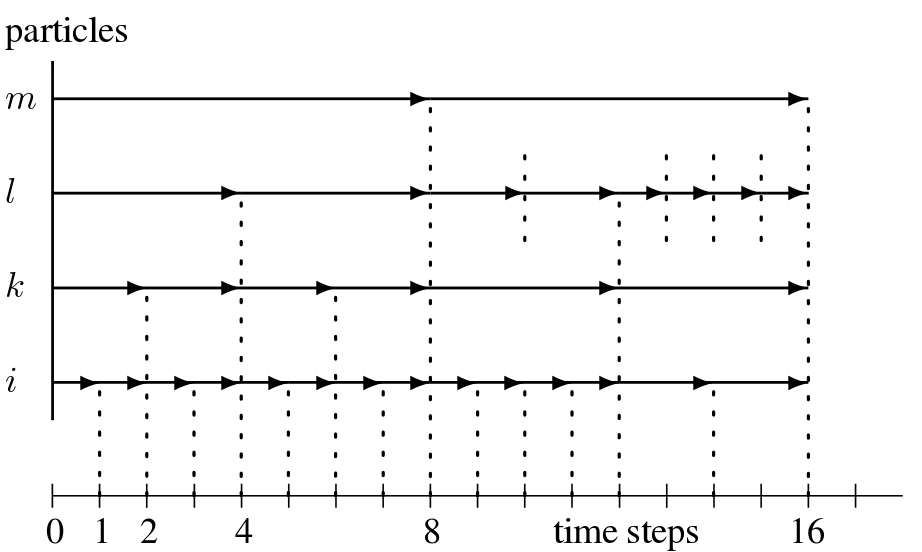
\includegraphics[width=0.6\linewidth]{Figures/0_block_timesteps.png}
\caption{Illustration of block time steps on 4 particles. Particles get their positions updated for each arrow symbol, common time steps are shown as vertical dotted lines. Figure from NB6++ User Manual. }
\end{figure} 
 
 
\subsection{KS-regularization}

Close binaries are extremely problematic in N-body simulations. They require a small time step as both binary components are much more accelerated than any other stars in the system, while the rest of the system is unaffected. Block time-step mitigate this problem, but the binary system still requires a lot of integration for an orbit that is essentially already known. Regularization is an answer to this problem. The essence of regularization is to decouple the integration of a sufficiently isolated sub-system, changing its coordinates to make integration easier, and including perturbations from external bodies. Several regularization scheme exist, NBODY6 implemented the Kustaanheimo-Stiefel method, or KS \citep{KS1965}.

Two bodies are candidates for regularization when their impact parameter is lower that the one needed for an orthogonal deviation, wherein their trajectory are deviated of 90$^\circ$:
\begin{equation}
b_\perp = 2G \frac{m_1 +m_2}{v^2_\infty}
\end{equation}
with $m_i$ components masses and $v_\infty$ relative velocity before encounter. This impact parameter can be converted to a time step computed through equation ~\ref{Eq:0_timestep}:
\begin{equation}
dt_{min} = \kappa \frac{\eta}{0.03} \left( \frac{r^3_{min}}{\langle m \rangle}\right)^\frac{1}{2}.
\end{equation}

To be actually regularized, two bodies have to have a mutual time step lower than $dt_{min}$ and fulfill two conditions:

\begin{align}
\bold{R_r} \cdot \bold{V_r} &> 0.1 \sqrt{ G(m_1+m_2)R_r}\\
\label{Eq:0_KSperturbation}
\frac{\left| \Delta \bold{F_r} \right| \cdot R^2_r}{G(m_1+m_2)} &< 0.25.
\end{align}

$\bold{R_r}$ and $\bold{V_r}$ being the relative velocities and positions of the particles and $\left| \Delta \bold{F_r} \right|$ the differential force applied to them, or perturbation. These conditions mean the subsystem is dynamically decoupled from external influence, but not unperturbed. When they are satisfied, the subsystem is regularized: it is replaced by the center of mass in the global system, and computed separately, with a set of changed coordinates. These coordinates are tailored for binary motion and close approach, they are well behaved when $R_r \rightarrow 0$. The influence of perturbers is taken into account when necessary. When the perturbation ratio (left hand side of equation~\ref{Eq:0_KSperturbation}) drops below a certain value, the system is considered isolated and it is not computed anymore, its parameters being stored until the perturbation is strong enough to warrant integration.

Regularisation have been extended to 3 and 4 bodies in hierarchical subsystems. NBODY6 can handle the regularization of a small-n non-hierarchical subsystem following the chain algorithm, see \cite{Mikkola1993}.


\subsection{Hermite integration scheme}

On the appropriate time-scales, the accelerations of the particles in a nbody system vary smoothly. It is therefore possible to predict the future acceleration then to correct the prediction, achivieving high order integration with limited computational cost. The Hermite integration scheme was first  introduced by \cite{Makino1991} and has since been implemented within NBODY6 \citep{Aarseth2003}.

%Using individual time steps, the standard integration algorithm starts by determining the next particle whose motion to integrate, that is the one whose integration step will bring us to the smaller time: $ i = min_j(t_j + \Delta t_j)$.

The first step is to compute the acceleration and its derivative at $t=t_0$ , for all particles $i$:

\begin{align}
\label{Eq:0_Hermite_acc1}
\bold{a}_{0,i} &= - \sum\limits_{i\neq j} G m_j \frac{\bold{R}}{R^3}\\
\label{Eq:0_Hermite_acc2}
\dot{\bold{a}}_{0,i} &=  - \sum\limits_{i\neq j} G m_j \left[ \frac{\bold{V}}{R^3}  + 
	\frac{ 3 \bold{R} ( \bold{V} \cdot \bold{R} )  }{R^3}\right]
\end{align}
with $\bold{R} = \bold{r}_{0,i} - \bold{r}_{0,j} $ and $\bold{V} = \bold{v}_{0,i} - \bold{v}_{0,j} $. Using these quantities, it is now possible to predict the positions and velocities at $t$ through a Taylor serie, again for all particles $i$:

\begin{align}
\bold{r}_{p,i}(t) &= \bold{r}_0 + \bold{v}_0 (t-t_0) + \bold{a}_{0,i}\frac{(t-t_0)^2}{2!} 	
		 +\dot{\bold{a}}_{0,i}\frac{(t-t_0)^3}{3!}\\
\bold{v}_{p,i}(t) &= \bold{v}_0 + \bold{a}_{0,i}(t-t_0) + \dot{\bold{a}}_{0,i}\frac{(t-t_0)^2}{2!}
\end{align}.

The predicted accelerations and their derivatives $\bold{a}_{p,i}(t)$,  $\dot{\bold{a}}_{p,i}(t)$ are computed by injecting $\bold{r}_{p,i}(t)$ and $\bold{v}_{p,i}(t)$ into equations \ref{Eq:0_Hermite_acc1} and \ref{Eq:0_Hermite_acc2}. The accelerations at t, of which predicted values have just been computed, can also be obtained through Taylor series:

\begin{align}
\label{Eq:0_Hermite_taylor1}
\bold{a}_{i}(t) &= \bold{a}_{0,i} + \dot{\bold{a}}_{0,i} (t-t_0) + \bold{a}^{(2)}_{0,i}\frac{(t-t_0)^2}{2!} + \bold{a}^{(3)}_{0,i}\frac{(t-t_0)^3}{3!}\\
\label{Eq:0_Hermite_taylor2}
\dot{\bold{a}}_{i}(t) &=  \dot{\bold{a}}_{0,i} +  \bold{a}^{(2)}_{0,i}(t-t_0) + \bold{a}^{(3)}_{0,i}\frac{(t-t_0)^2}{2!}
\end{align}
with $\bold{a}^{(2)}_{0,i}$,$\bold{a}^{(3)}_{0,i}$ the third and fourth derivative of the acceleration at $t=0$. Note that these quantities are unknown for now. To take the derivatives of equation \ref{Eq:0_Hermite_acc2} would be too computationnaly expansive. Instead, $\bold{a}_{p,i}(t)$ and  $\dot{\bold{a}}_{p,i}(t)$ are injected in the left hand side of equations \ref{Eq:0_Hermite_taylor1} and \ref{Eq:0_Hermite_taylor2} and solved for $\bold{a}^{(2)}_{0,i}$ and $\bold{a}^{(3)}_{0,i}$. This leads to the expressions:

\begin{align}
\bold{a}^{(3)}_{0,i} &= 12 \frac{\bold{a}_{0,i} - \bold{a}_{p,i}}{(t-t_0)^3} +6 \frac{\dot{\bold{a}}_{0,i} - \dot{\bold{a}}_{p,i}}{(t-t_0)^3}\\
\bold{a}^{(2)}_{0,i} &= -6 \frac{\bold{a}_{0,i} - \bold{a}_{p,i}}{(t-t_0)^2} - 2 \frac{2\dot{\bold{a}}_{0,i} + \dot{\bold{a}}_{p,i}}{t-t_0}.
\end{align}

The predicted values of positions and velocities are then corrected using the second and third order derivatives of acceleration, yeilding fifth order accurate values.

\begin{align}
\bold{r}_{c,i}(t) &= \bold{r}_{p,i}(t) + \bold{a}^{(2)}_{0,i} \frac{(t-t_0)^4}{4!} +
	 \bold{a}^{(3)}_{0,i} \frac{(t-t_0)^5}{5!}\\
\bold{v}_{c,i}(t) &= \bold{v}_{p,i}(t) + \bold{a}^{(2)}_{0,i} \frac{(t-t_0)^3}{3!} +
	 \bold{a}^{(3)}_{0,i} \frac{(t-t_0)^4}{4!}\\
\end{align}

In a nutshell, the Hermite scheme is a way to obtain 5th order terms with limited cost. First $r_0^{(2)}$ and $r_0^{(3)}$ are computed, then used to obtain predictions of $r_t^{(0)}$ and $r_t^{(1)}$, transformed with the equations of motions into predictions of $r_t^{(3)}$ and $r_t^{(4)}$. These last two can be expressed through Taylor series as functions of $r_0^{(3)}$,$r_0^{(4)}$ and $r_0^{(5)}$, which are solved for these last two terms. The predicted values of $r_t^{(0)}$ and $r_t^{(1)}$ are then corrected to the fifth order with $r_0^{(4)}$ and $r_0^{(5)}$.

The error for a single time step scales as $O(\Delta t^5)$. The Hermite scheme has shown itself very well suited for the block time step method, as the synchronization of particles limit the amount of prediction to be made, many positions at a given time being already known and computed with maximum accuracy.


\subsection{Ahmad-Cohen neighbour scheme}

For a given particle in an nbody system, the influence of direct neighbours changes on shorter timescales than the smooth potential from distant particles. The essence of the Ahmad-Cohen neighbour scheme is to decouple the two for computational efficiency \citep{AhmadCohen1973}. The acceleration is splitted into two components:

\begin{equation}
\bold{a}_i = \bold{a}_{i,reg} + \bold{a}_{i,irr}
\end{equation}

$\bold{a}_{i,irr}$ is the acceleration from particles inside a given "neighbour sphere" around particle $i$, while $\bold{a}_{i,reg}$ is the acceleration from all other, more distant, particles. Integration within the neighbours sphere,  \textit{irregular} integration, is decoupled from the global, \textit{regular}, integration. Regular time steps, where complete force summation are performed over all particles with eq \ref{Eq:0_Hermite_acc1}, are subdivided into irregular time steps, where regular acceleration is predicted and irregular acceleration is computed through a force summation on the $N_{i,nb}$ neighbours. The list of neighbours of $i$ is updated every regular time step and contains the particles within a sphere of radius $R_{i,s}$ centered on $i$. Are also added to the neighbour list are the particles within $2^{\frac{1}{3}}R_{i,s} $ that satisfy the condition
\begin{equation}
\bold{R} \cdot \bold{V} < 0.1 \frac{R_s^2}{\Delta T_{reg}}
\end{equation}
with $\Delta T_{reg}$ the regular time step. This ensures that fast approaching particles are selected before they enter the actual neighbour sphere. $R_{i,s}$ is determined through local number density contrast and optimisation of the resulting $N_{i,nb}$. 

When $N_{nb} \ll N$ for most particles, there is a great performance improvement, without loss of accuracy. 



\newpage
 \section{Young star clusters}











